\section{A Model Problem}
\label{sec:ginzburg_landau}

The asymptotic center-manifold derived in section~\ref{sec:center_manifold_derivation} is applied to a Ginzburg-Landau model which is described by a complex-conjugate pair of equations as,
\begin{subequations}
	\label{eqn:ginzburg_landau}
	\begin{align}
		\dfrac{\partial A}{\partial t} =& \left[\delta_{1}\dfrac{\partial}{\partial x} + \delta_{2} + \delta_{3}x + \delta_{4}\dfrac{\partial^{2}}{\partial x^{2}}\right]A - \delta_{5}|A|^{2}A, \\
		%
		\dfrac{\partial A^{*}}{\partial t} =& \left[\delta^{*}_{1}\dfrac{\partial}{\partial x} + \delta^{*}_{2} + \delta^{*}_{3}x + \delta^{*}_{4}\dfrac{\partial^{2}}{\partial x^{2}}\right]A^{*} - \delta^{*}_{5}|A|^{2}A^{*}. 
	\end{align}
\end{subequations}
Where, $x$ is the spatial coordinate and the superscript $^{*}$ represents complex conjugation. Typically such a model would arise as the simplified dynamics of a more detailed dynamical system. Here the Ginzburg-Landau model itself is treated as the underlying dynamical model. Such models have often been utilized to investigate local and global bifurcations in spatially developing flows \citep{chomaz88,chomaz05}. For $A=0$ at the left and right domain boundaries, it is easily seen that $A(x)=0$ identically represents a fixed point of the system, with the linear operators given by
\begin{align}
	\mathcal{L}_{0}	=& \left[\delta_{1}\dfrac{\partial}{\partial x} + \delta_{2} + \delta_{3}x + \delta_{4}\dfrac{\partial^{2}}{\partial x^{2}}\right], \nonumber \\
	%
	\mathcal{L}^{*}_{0} =&\left[\delta^{*}_{1}\dfrac{\partial}{\partial x} + \delta^{*}_{2} + \delta^{*}_{3}x + \delta^{*}_{4}\dfrac{\partial^{2}}{\partial x^{2}}\right], \nonumber
\end{align}
and the linear operator for both $A$ and $A^{*}$ written together as
\begin{eqnarray}
	\mathcal{L} = \begin{bmatrix}
		\mathcal{L}_{0}		& 0 \\
		0								  & \mathcal{L}^{*}_{0}
	\end{bmatrix}
\end{eqnarray}

For semi-infinite domains, $x\in[0,\infty)$, the spectrum for $\mathcal{L}_{1}$ is known analytically \citep{chomaz88} and is given by,
%\begin{subequations}
	\begin{align}
		\omega_{n}	=& \delta_{2} - \dfrac{\delta_{1}^{2}}{4\delta_{4}} + (\delta_{4}\delta_{3}^{2})^{1/3}\zeta_{n}, \label{eqn:eigenvalues} 
		%
		%\phi_{n}(x)		=& \mathrm{Ai}([-\delta_{3}/\delta_{4}]^{1/3}x + \zeta_{n}), \label{eqn:eigenvectors}
	\end{align}
%\end{subequations}
and the corrresponding complex conjugate for $\mathcal{L}^{*}_{0}$. Here $\mathrm{Ai}$ denotes the Airy function and $\zeta_{n}$ its countable set of zeros.
 The system parameters at bifurcation are chosen \emph{ad hoc} as $\delta^{0}_{1} = -1.0$, $\delta^{0}_{2} = 0.741 + 1.025i$, $\delta^{0}_{3}=0.125$, $\delta^{0}_{4}=(1.0 - i)/\sqrt{2}$ and $\delta^{0}_{5} = $, which results in a single critical eigenmode with eigenvalue $\omega_{c} = 1.0i$ for $\mathcal{L}_{0}$ and its conjugate, $-1.0i$ for $\mathcal{L}^{*}_{0}$, and all other eigenvalues have negative real parts. 
 
 A center-manifold approximation of the model problem requires the evaluation of restricted resolvents, which is a difficult problem to solve analytically. Therefore the problem is considered in a trucated domain of $x\in [0,40]$ with the boundary conditions of $A = 0$ at $x=0$ and, $\partial A/\partial x = 0$ at $x=40$. Due to the spatially localized nature of the first few eigenvectors (which dictate the global dynamics), this truncation does not affect the dynamics in any significant manner, as can be seen from the comparison between the analytical spectrum of the semi-infinite domain, and the first five numerically calculated eigenvalues in the truncated domain in figure~\ref{fig:GL_spectrum}. The numerical spectrum was obtained via the implicitly restarted Arnoldi method \citep{sorensen92}. 
\begin{figure}
	\centering
	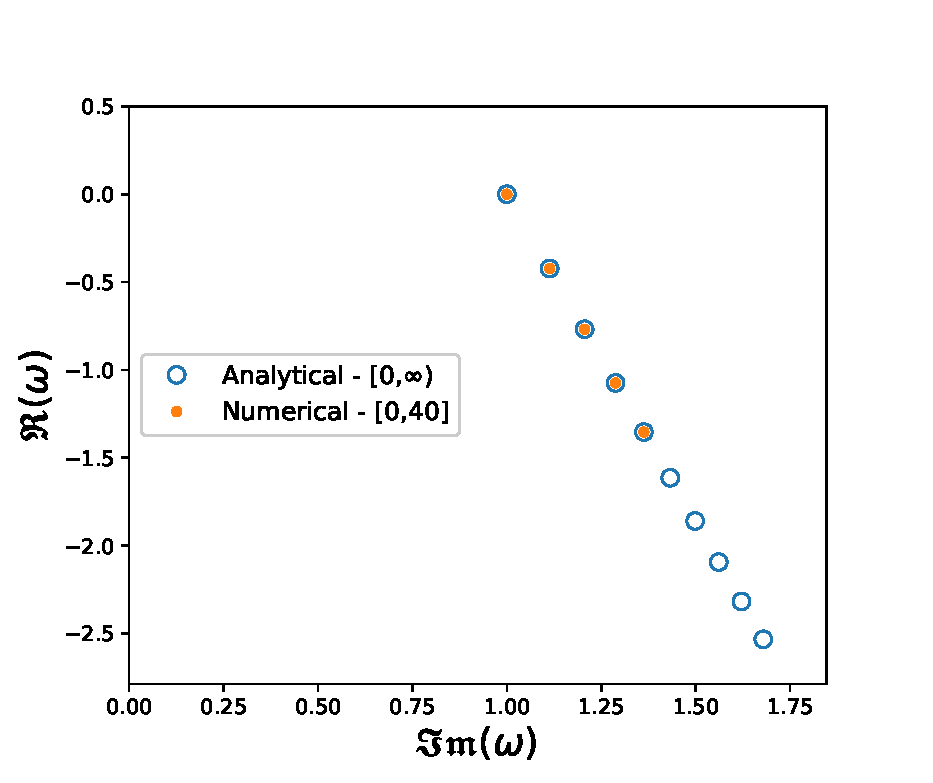
\includegraphics[width=0.49\textwidth]{GL_spectra}
	\caption{Comparison of the numerically evaluated spectrum of the Ginzburg-Landau model $(\mathcal{L}_{0})$ in the truncated domain with the analytical spectrum in the semi-infinite domain.}
	\label{fig:GL_spectrum}
\end{figure}

The structure of the eigenmodes is given by,
 \begin{align}
	\vecv_{5} = \begin{Bmatrix}
		\phi_{c} \\
		0 
	\end{Bmatrix}, & \hspace{2mm}
	%
	\vecv_{6} = \begin{Bmatrix}
		0 \\
		\phi^{*}_{c} 
	\end{Bmatrix}, \nonumber
\end{align}
where, $(\omega_{c},\phi_{c})$ and $(\omega^{*}_{c},\phi^{*}_{c})$ are the critical eigenpairs of $\mathcal{L}_{0}$ and $\mathcal{L}^{*}_{0}$ respectively. Similarly, the adjoint eigenmodes are denoted as,
\begin{align}
	\vecw_{5} = \begin{Bmatrix}
		\chi_{c} \\
		0 
	\end{Bmatrix}, & \hspace{2mm}
	%
	\vecw_{6} = \begin{Bmatrix}
		0 \\
		\chi^{*}_{c} 
	\end{Bmatrix}, \nonumber
\end{align}
where, $(\omega^{*}_{c},\chi_{c})$ and $(\omega_{c},\chi^{*}_{c})$ are the eigenpairs of corresponding adjoint linear operators $\mathcal{L}^{\dagger}_{0}$ and $\mathcal{L}^{*\dagger}_{0}$ respectively. The projection operator into the stable subspace of $\mathcal{L}$ is defined as
\begin{align}
	\mathbf{Q} = \mathbf{I} - \vecv_{5}\vecw_{5}^{H} - \vecv_{6}\vecw_{6}^{H}. \nonumber
\end{align}
The projectors into the stable subspaces of $\mathcal{L}_{0}$ and $\mathcal{L}^{*}_{0}$ are denoted as $\mathbf{Q}_{0}$ and $\mathbf{Q}^{*}_{0}$, and are given by,
\begin{align}
	\mathbf{Q}_{0} 			=& \mathbf{I} - \phi_{c}\chi^{H}_{c}, & 
	\mathbf{Q}^{*}_{0} 	=& \mathbf{I} - \phi^{*}_{c}\chi^{*H}_{c}. \nonumber
\end{align}

The system in equation~\eqref{eqn:ginzburg_landau} has a total of five parameters (ten including the complex-conjugate pairs) that can be varied from their bifurcation values. In order to avoid an explosion in the number of terms $T_{k}$ arising from the combinatorial problem, only the variations in $\delta_{3},\delta_{4},\delta^{*}_{3}$ and $\delta^{*}_{4}$ are considered, which suffice to illustrate the derivation of the asymptotic center-manifold under parameter variations. Although the parameters are complex-conjugate pairs, it turns out to be simplest to treat them all as independent parameters and enforce the complex-conjugate property later when parameter values are prescribed. The extended variable for the parameter evolution is then $\vecnu = [\delta'_{3};\delta'_{4};\delta'^{*}_{3};\delta'^{*}_{4}]$, with 
\begin{align}
	\delta_{3} =& \delta^{0}_{3} + \delta'_{3},& \delta_{4} =& \delta^{0}_{4} + \delta'_{4}, \nonumber \\
	\delta^{*}_{3} =& (\delta^{0}_{3})^{*} + \delta'^{*}_{3}, &\delta^{*}_{4} =& (\delta^{0}_{4})^{*} + \delta'^{*}_{4}. \nonumber
\end{align}
The extended state vector is denoted as $\widehat{A} = [A; A^{*}; \vecnu]$. With the knowledge of the linear operator and having calculated the critical eigenmodes, all the terms for the center-manifold approximation can be now be easily built. 
The extended linear operator is given by,
 \begin{align}
 	\mathcal{\widehat{L}} = \begin{bmatrix}
 		\mathcal{L}_{0} 	   &	0										&	0 \\
 		0									  & \mathcal{L}^{*}_{0}		&   0 \\
 		0									  & 0											&  0
 	\end{bmatrix}. \nonumber
 \end{align}
This results in six critical modes for the extended system - two critical modes resulting from the original linear system $\mathcal{L}$ and four parameter modes due to system extension. The structure of the critical modes is given by
 \begin{align}
	\widehat{\vecv}_{i} = \begin{Bmatrix}
		0 \\
		0 \\
		\vfield{e}_{i}
	\end{Bmatrix}, & \hspace{2mm} \text{for } i \in 1,2,3,4 \nonumber \\
	%
	\widehat{\vecv}_{5} = \begin{Bmatrix}
		\phi_{c} \\
		0 \\
		0
	\end{Bmatrix}, & \hspace{2mm}
	%
	\widehat{\vecv}_{6} = \begin{Bmatrix}
		0 \\
		\phi^{*}_{c} \\
		0
	\end{Bmatrix}, \nonumber
\end{align}
with the adjoint critical modes defined by,
 \begin{align}
	\widehat{\vecw}_{i} = \begin{Bmatrix}
		0 \\
		0 \\
		\vfield{e}_{i}
	\end{Bmatrix}, & \hspace{2mm} \text{for } i \in 1,2,3,4 \nonumber \\
	%
	\widehat{\vecw}_{5} = \begin{Bmatrix}
		\chi_{c} \\
		0 \\
		0
	\end{Bmatrix}, & \hspace{2mm}
	%
	\widehat{\vecw}_{6} = \begin{Bmatrix}
		0 \\
		\chi^{*}_{c} \\
		0
	\end{Bmatrix}. \nonumber
\end{align}
The matrices $\mathbf{\widehat{V}}$ and $\mathbf{\widehat{W}}$ are defined accordingly.
The nonlinear term is given by
\begin{align}
	\vecf_{NL} = \begin{Bmatrix}
		\vecf^{1}_{NL} \vspace{1mm}\\
		\vecf^{2}_{NL}
	\end{Bmatrix} = 	
	\begin{Bmatrix}
		\delta'_{3}xA + \delta'_{4}(\partial^{2}A/\partial x^{2}) + \delta^{0}_{5}|A|^{2}A	\vspace{1mm} \\
		(\delta'_{3}xA + \delta'_{4}(\partial^{2}A/\partial x^{2}) + \delta^{0}_{5}|A|^{2}A)^{*}
	\end{Bmatrix}, \nonumber
\end{align}
and the reduced system matrix $\mathbf{\widehat{K}}$ is then given by
\begin{align}
	\mathbf{\widehat{K}} = \begin{bmatrix}
		0 & 0 & 0 & 0 & 0& 0 \\ 
		0 & 0 & 0 & 0 & 0& 0 \\ 
		0 & 0 & 0 & 0 & 0& 0 \\ 
		0 & 0 & 0 & 0 & 0& 0 \\ 
		0 & 0 & 0 & 0 & \omega_{c} & 0 \\ 
		0 & 0 & 0 & 0 & 0 & \omega^{*}_{c}
	\end{bmatrix}. \nonumber
\end{align}
Due to the absence of purely real critical eigenvalues in the original system, the $\Gammabf$ matrix vanishes and hence the coupling terms $\vecg^{c}_{\alpha,\beta}$ vanish identically. 
To avoid confusion with the spatial variable $x$, the critical mode amplitudes are denoted by $\zbf = [z_{1};z_{2};z_{3};z_{4};z_{5};z_{6}]$, the stable component solution of the original system is given by $A_{s} = [A^{1}_{s}; A^{2}_{s}]$, and in the extended space it is $\widehat{A}_{s} = [A^{1}_{s}; A^{2}_{s}; 0]$. Thus the total solution is written as,
\begin{eqnarray}
	\widehat{A} = \widehat{\mathbf{V}}\zbf + \widehat{A}_{s}. \nonumber
\end{eqnarray}
With all the subcomponents evaluated, the center-manifold theorem may be applied to the extended system and the stable component solution evaluated asympotically as
\begin{align}
	\label{eqn:GL_asymptotic}
		\mathfrak{h}(\mathbf{z}) =& \sum_{a=1}^{6}\sum_{b=a}^{6} z_{a}z_{b}\vfield{y}_{a,b}
		 + \mathcal{O}(\mathbf{z}^{3}), \nonumber \\
		 %
		 \vfield{y}_{a,b} =& \begin{Bmatrix}
		 	\vfield{y}^{1}_{a,b} \vspace{1mm} \\
		 	\vfield{y}^{2}_{a,b}
		 \end{Bmatrix}.	\nonumber
\end{align}
For $M=6$, one obtains a total of $T_{2}=21$ terms at second order for the asymptotic approximation. However most of these terms vanish and one obtains the following expressions for the forcing terms $\vecg_{\alpha,\beta}$,
\begin{align}
	\vecg_{1,1}  = \vecg_{1,2} = \vecg_{1,3}  = \vecg_{1,4} = \vecg_{1,6} = \emptyset, \nonumber \\
	\vecg_{2,2} = \vecg_{2,3} = \vecg_{2,4} = \vecg_{2,6} = \emptyset, \nonumber \\
	\vecg_{3,3} = \vecg_{3,4} = \vecg_{3,5} = \emptyset, \nonumber \\
	\vecg_{4,4} = \vecg_{4,5} = \emptyset, \nonumber \\
	\vecg_{5,5} = \vecg_{5,6} = \vecg_{6,6} = \emptyset, \nonumber
\end{align}
and,
\begin{align}
	\vecg_{1,5} =& 	\mathbf{Q}\cdot x\vecv_{5} =&
	\begin{Bmatrix}
		\mathbf{Q}_{0}x\phi_{c} \\
		0
	\end{Bmatrix}, \nonumber \\
	%
	\vecg_{2,5} =& 	\mathbf{Q}\cdot \dfrac{\partial^{2}\vecv_{5}}{\partial x^{2}} =&
	\begin{Bmatrix}
		\mathbf{Q}_{0}\partial^{2}\phi_{c}/\partial x^{2}	\\
		0
	\end{Bmatrix}, \nonumber \\
	%
	\vecg_{3,6} =& 	\mathbf{Q}\cdot x\vecv_{6} =&
	\begin{Bmatrix}
		0	\\
		\mathbf{Q}^{*}_{0}x\phi^{*}_{c}
	\end{Bmatrix}, \nonumber \\
	%
	\vecg_{4,6} =& 	\mathbf{Q}\cdot \dfrac{\partial^{2}\vecv_{6}}{\partial x^{2}} =&
	\begin{Bmatrix}
		0	\\
		\mathbf{Q}^{*}_{0}\partial^{2}\phi^{*}_{c}/\partial x^{2}
	\end{Bmatrix}. \nonumber
\end{align}
 which results in the restricted resolvent solutions that satisfy,
 \begin{subequations}
 	\label{eqn:GL_resolvents}
	 \begin{align}
	 	\mathbf{Q}[(0 + \omega_{c})\mathbf{I} - \mathcal{L}]\mathbf{Q}\vecy_{1,5} =& \vecg_{1,5}, \\
	 	%
	 	\mathbf{Q}[(0 + \omega_{c})\mathbf{I} - \mathcal{L}]\mathbf{Q}\vecy_{2,5} =& \vecg_{2,5}, \\
	 	%
	 	\mathbf{Q}[(0 + \omega^{*}_{c})\mathbf{I} - \mathcal{L}]\mathbf{Q}\vecy_{3,6} =& \vecg_{3,6}, \\
	 	%
	 	\mathbf{Q}[(0 + \omega^{*}_{c})\mathbf{I} - \mathcal{L}]\mathbf{Q}\vecy_{4,6} =& \vecg_{4,6}. 
	 \end{align}
\end{subequations}
The resolvent solutions in terms of the individual fields are written as
 \begin{subequations}
 	\label{eqn:GL_sub_resolvents}
	 \begin{align}
	 	\mathbf{Q}_{0}[(0 + \omega_{c})\mathbf{I} - \mathcal{L}_{0}]\mathbf{Q}_{0}\vecy^{1}_{1,5} =& \mathbf{Q}_{0}x\phi_{c}, \\
	 	%
	 	\mathbf{Q}_{0}[(0 + \omega_{c})\mathbf{I} - \mathcal{L}_{0}]\mathbf{Q}_{0}\vecy^{1}_{2,5} =& \mathbf{Q}_{0}\dfrac{\partial^{2}\phi_{c}}{\partial x^{2}}, \\
	 	%
	 	%
	 	\mathbf{Q}^{*}_{0}[(0 + \omega^{*}_{c})\mathbf{I} - \mathcal{L}^{*}_{0}]\mathbf{Q}^{*}_{0}\vecy^{2}_{3,6} =& \mathbf{Q}^{*}_{0}x\phi^{*}_{c}, \\
		%
		\mathbf{Q}^{*}_{0}[(0 + \omega^{*}_{c})\mathbf{I} - \mathcal{L}^{*}_{0}]\mathbf{Q}^{*}_{0}\vecy^{2}_{2,5} =& \mathbf{Q}^{*}_{0}\dfrac{\partial^{2}\phi^{*}_{c}}{\partial x^{2}}.
		%
	 \end{align}
\end{subequations}
 Obviously, $\vecy^{2}_{3,6} = (\vecy^{1}_{1,5})^{*}$ and $\vecy^{2}_{4,6} = (\vecy^{1}_{2,5})^{*}$, as would be expected from the original equations. 
 


%The asympotic formulation derived in the previous sections is applied to the case of the first bifurcation of a cylinder wake. The bifurcation problem has been investigated by several authors in various settings \citep{provansal87,dusek94,pier02,barkley06,giannetti07,sipp07,mantivc15,negi20}. The problem is revisited in the context of a center manifold approximation which is valid in the vicinity of the bifurcation point. 
%
%The investigation is carried out numerically using Nek5000, an open source fluid dynamics solver originating at Argonne National Laboratory \citep{nek5000}. The code implements the spectral element method \citep{patera84}  for the Navier--Stokes equations with the $\mathds{P}_{n}-\mathds{P}_{n-2}$ formulation \citep{maday89}. The current work uses ninth order Lagrange polynomials in each direction for the representation of velocities in each spectral element and a seventh order Lagrange polynomial for the pressure with a total of $3760$ elements in the whole domain. Time integration of the system is performed using a third-order backward difference scheme with an implicit treatment of the viscous term. The non-linear terms are evaluated explicitly using extrapolation. Incompressibility is enforced using the pressure projection method \citep{deville02} implemented through the inexact LU factorization. Numerical stabilization is done using the HPF-RT method \citep{negiphd}, which adds a small amount of dissipation at the highest wavenumber scales. All quantities are non-dimensionalized using the fluid density $\rho$, the cylinder diameter $D$ and the inflow velocity $U$. The flow is characterized by the Reynolds number defined as $\Rey = UD/\nu$, where $\nu$ is the kinematic viscosity of the fluid. 
%
%The problem domain is set up with the cylinder center located at the origin, the inflow boundary located at $x=-20$, the outflow boundary located at $x=40$ and far field boundaries located at $y=\pm20$. Dirichlet boundary condition is specified at the inflow and the standard no-stress boundary condition is applied at the outflow. The far-field boundary is equipped with the symmetry boundary condition. The bifurcation point of the system is found via a combination of selective fequency damping \citep{akervik06} for determining the fixed point of the system at each $\Rey$, along with a bisection-like algorithm for determining the point with zero growth rate. The spectral problem was solved using the Krylov-Schur algorithm \citep{stewart02}. The details of the procedure may be found in Appendix B.
%
%The critical Reynolds number is found to be $\Rey_{c} = 46.30$ which is close to the value of $46.6$ reported in the work of \cite{sipp07}. The spectrum obtained at the bifurcation point is depicted in figure~\ref{fig:cyl_spectrum}, including the parameter mode located at the origin. The streamwise velocity for the calculated baseflow along with the parameter mode due to the extension of the system is depicted in figure~\ref{fig:base_param}. The complex conjugate pair of critical eigenvalues for the baseflow is found to be $\lambda_{c} = \pm0.7456i$, which compares well with $\lambda_{c}=\pm0.74i$ reported in \cite{sipp07}. The direct and adjoint critical eigenmodes of the flow are shown in figures~\ref{fig:flowconfig} and ~\ref{fig:flowconfig_2} respectively. The complex-conjugated mode is not shown. The modes are normalized such that the direct modes are of unit norm and the adjoint modes are scaled appropriately to maintain biorthogonality. The parameter mode is the exception where the normalization is such that $\zeta^{\dagger}_{0} = \zeta_{0} = 1$.
%
%Once the fields $\vpfield{y}_{i,j}$ have been evaluated, substitution in to equation~\eqref{amplitude_second_oder} then results in the coefficients of the polynomial terms $x_{i}x_{j}$ and $x_{i}x_{j}x_{k}, \ (i,j,k \in 0,1,2;\ j\ge i; k\ge j)$ of the center-manifold amplitude equations. When the graph equation is evaluated asymptotically at second order the resulting center-manifold equations are of third order (in $\mathbf{x}$). Since $x_{1}$ and $x_{2}$ are the amplitudes of the complex-conjugated pair of modes, the resulting expressions for the center-manifold amplitude equations obtained for the two variables are also complex-conjuated with respect to the other. Differences arise due to the numerical accuracy of the terms evaluated and in the current work this complex-conjugacy property is violated at $\mathcal{O}(10^{-8})$. A full list of the evaluated terms is given in the appendix. The combinatorial problem would allow a total of $19$ terms for each equation however, a significant number of the terms are of the order of the convergence tolerance used for the spectral solver and are treated as negligible. Even the inhomogeneous terms $x_{0}x_{0}$ and $x_{0}x_{0}x_{0}$ are negligible in the current case under examination. The vanishing of several terms in the center-manifold amplitude equations may also be deduced by inspecting the spatial symmetry of the resulting terms. Replacing $x_{1},x_{2}$ with $x,x^{*}$, and $x_{0}$ with the parameter variable $\eta$, and ignoring the small terms ($<10^{-5}$), one obtains the following equation for $\dt{x}$
%\begin{equation}
%	\label{numerical_amplitude_eqn_x1_p1}
%	\begin{aligned}
%			\dt{x} =& +[0.7456i]x \\
%			%
%			& + [(1.976 + 0.698i)\times10^{-1}]\eta x \\ 
%			%
%			& + [(6.388 + 4.616i)\times10^{-3}]\eta x^{*}  \\
%			%
%			& + [(7.264 - 4.787i)\times10^{-2}]\eta^{2} x \\
%			%
%			& + [(4.477 - 1.482i)\times10^{-3}]\eta^{2}x^{*} \\
%			%
%			& + [(1.615 - 2.904i)\times10^{-5}]x^{3}  \\
%			%
%			& - [(2.526 - 8.010i)\times10^{-3}](x^{*}x)x \\
%			%
%			& + [(0.973 - 3.380i)\times10^{-5}](x^{*}x)x^{*} \\
%			%
%		\end{aligned}
%\end{equation}
%The complex conjugation of equation~\eqref{numerical_amplitude_eqn_x1_p1} results in the equation for $\dt{x}^{*}$. The equation may now be evaluated numerically to obtain the time history and the resulting non-linear angular frequency of the reduced system. The evolution of the system at a parameter value of $\eta=0.074$ ($\Rey=50.0$) is shown in figure~\ref{fig:center_manifold_evolution}, depicting the typical evolution to the saturated limit cycle. 
%
%The center-manifold amplitude equations are numerically integrated for several different parameter values and the angular frequency of the limit cycle oscillations is obtained. The comparison between the frequencies obtained through the full non-linear simulations and those obtained through the reduced center-manifold amplitude equations is show in figure~\ref{fig:limit_cycle_frequency}. Close to the bifurcation point the saturated limit-cycle frequencies are well predicted by the reduced equations however, as the Reynolds number increases the saturation frequency systematically deviates from the results of the full non-linear simulations. Recall that the the center-manifold reduction is only an asymptotic approximation, therefore higher order terms could provide contributions as the system is moved away from the critical point. Alternately, the center-manifold approximation itself may not be valid sufficiently far away from the critical point, so that the solution $\vpfield{u}_{s}$ which lies in the stable subspace can no longer be assumed to evolve as a graph of the critical subspace. 
%
%In addition to the saturated limit cycle angular frequency one may also estimate the variation of the linearized angular frequency \ie the eigenvalue of system beyond the critical point through the reduced equations. Since the inhomogeneous terms in the reduced system are negligible, the variation of the eigenvalue as a function of the parameter $\eta$ is directly obtained from the linear terms  in equation~\eqref{numerical_amplitude_eqn_x1_p1}. A comparison of the obtained eigenfrequencies of the center-manifold equations ($\mathcal{O}(\mathbf{x}^{3})$) and those computed for the full system using the Krylov-Schur algorithm for different Reynolds numbers is shown in figure~\ref{fig:linearized_eigenvalue}. Close to the critical point the variation of the eigenvalue seems to be fairly well captured by the reduced equations. In an attempt to obtain a better asymptotic approximation higher order terms up to $\mathcal{O}(\mathbf{x}^{4})$ were evaluated resulting in a fifth order equation for the center-manifold amplitudes. However, at this order the highest order term $(|x|^{4}x)$ has a coefficient with a positive real part, leading to an unbounded system. Presumably one needs to evaluate $\mathfrak{h}(\mathbf{x})$ to $\mathcal{O}(\mathbf{x}^6)$ to obtain a bounded reduced system again (in which case the center-manifold amplitude equations would be of $\mathcal{O}(\mathbf{x}^{7})$). Further higher order approximations have not been pursued. One may nonetheless obtain a higher-order estimate of the linearized frequencies of the reduced system from this higher order (but unbounded) system ($\mathcal{O}(\mathbf{x}^{5})$). This is plotted in figure~\ref{fig:linearized_eigenvalue} with a dashed line. Clearly the higher order estimate follows the eigenvalues of the full system much more closely, providing evidence for the conjecture that the higher order terms of the asymptotic approximation do indeed have significant contribution as the system moves away from the critical point.
%
%\subsection{The Stuart-Landau equation}
%\label{stuart_landau}
%
%The Landau model has often been utilized to understand the behavior of weakly unstable systems close to the bifurcation point \citep{dusek94,sipp07,carini15,meliga12}. The original model was proposed by Landau based on symmetry, scaling and phenomenological arguments \citep{landau_52}. In the hydrodynamics literature the model is referred to as the Stuart-Landau equation and was first obtained through energy considerations in \cite{stuart58} and via the separation of time scales in \cite{stuart60,watson60}. In order to transform the center-manifold amplitude equations to a form similar to the Stuart-Landau equation, one may multiply equation~\eqref{numerical_amplitude_eqn_x1_p1} with $x^{*}$, and multiply the the complex-conjugate of equation~\eqref{numerical_amplitude_eqn_x1_p1} with $x$. Adding the two resulting equations together leads to an equation for the squared amplitude $x^{*}x = |x|^{2}$. One may then follow the phenomenological arguments of \cite{landau_52} for the evolution of the amplitudes in the case of small linear growth rates. Assuming that the system is close to the bifurcation point and the instability is weak, then the change in the amplitude over one cycle of the fundamental frequency also remains small. In such a scenario the evolution equation for the squared amplitude may be averaged over one cycle to obtain the evolution of the average amplitude. The averaging process causes all the oscillatory terms of the type $(x)^{2},(x^{*})^{2},|x|^{2}(x),|x|^{2}(x^{*})$ \textit{etc.} to (nearly) vanish, and the only remaining terms are those related to the modulus of the amplitude. Representing the averaged modulus as $|A|^{2} = \overline{|x|^{2}}$, one obtains the Landau model for the problem as
%\begin{equation}
%	\label{landau_eqn_1}
%		\dfrac{d|A|^{2}}{dt} = 2\times[0.1976\eta + 0.0726\eta^{2}] |A|^{2} - 0.0051|A|^{4}.
%\end{equation}
%The arguments presented by Landau correspond to the more formal procedure of multiple time-scale expansion and the averaged amplitude $|A|$ corresponds to the amplitude modulation governed by the slow time-scale equations (usually obtained through the solvability condition).
%
%While this is not undertaken in the original work of \cite{landau_52}, a similar procedure may be invoked to obtain a slow drift of the angular frequency. Representing $x = |A|e^{i\theta} = |A|e^{i\phi(t)}e^{\lambda_{c}t}$, where, $\phi(t)$ represents the slowly varying drift in angular frequency and $\lambda_{c}$ the critical eigenvalue of the system. One may substitute this expression into equation~\eqref{numerical_amplitude_eqn_x1_p1} and subtract the complex conjugated equation (corresponding to the equation for $x^{*}$) to obtain an expression for $\dt{\phi}$. This equation again contains oscillatory terms of the type $e^{\lambda_{c}t},e^{-\lambda_{c}t},e^{2\lambda_{c}t},e^{-2\lambda_{c}t}$ \textit{etc}. These may be eliminated by averaging over the fundamental time period of the oscillation, with the assumption that $\phi(t)$ remains nearly constant during one cycle of the oscillation, resulting in the expression,
%\begin{equation}
%	\label{landau_eqn_2}
%	\dfrac{d\phi}{dt} = [0.0698\eta - 0.0478\eta^{2}]  + 0.0080|A|^{2}.
%\end{equation}
%Combining the two equations in $A = |A|e^{i\phi(t)}$ and using the definition of the derivatives in equations~\eqref{landau_eqn_1} and \eqref{landau_eqn_2} one obtains
%\begin{eqnarray}
%	\label{stuart_landau_eqn}
%	\begin{split}
%		\dt{A} 					=& [(0.1976 + i0.0698)\eta + (0.0726 - i0.0478)\eta^{2}] A \\
%										& - \frac{1}{2}[0.0051 - i0.0160]|A|^{2}A.
%	\end{split}
%\end{eqnarray}
%This is the amplitude equation or, the Stuart-Landau equation for the case in question. In its normal form the Stuart-Landau equation is represented as $\dt{A} = (\sigma_{r} + i\sigma_{i})A - 1/2(l_{r} + il_{i})|A|^{2}A$, and the correspondence is seen immediately. Equation~\eqref{stuart_landau_eqn} may be derived more formally through the usual procedure of multiple time-scale expansion. This however is not undertaken and the phenomenological arguments are deemed sufficient, especially given that a reduced system of center-manifold amplitude evolution has already been obtained in equation~\eqref{numerical_amplitude_eqn_x1_p1}. The Landau constant is found to be $l_{r} = 0.0051$, however, this constant depends on the normalization of the global mode. The ratio $l_{i}/l_{r} = -3.14$ is independent of the normalization. There appears to be some amount of scatter in the reported values of this ratio in the literature, with reported value being $-2.7$  in \cite{dusek94}, $-3.42$ in \cite{sipp07}, $-3.3$ in \cite{meliga12}, and $-3.63$ in \cite{carini15}. The value found in the current work seems to be within the scatter reported in the literature and the reasons behind the scatter are not entirely clear. The ``growth-rate'' of the amplitude that varies linearly with $\eta$ is found here to be $\sigma_{r}=0.1976$ which at first glance appears to be very different from the values reported in \cite{sipp07,meliga12,carini15}. However, in the current work $\eta$ is scaled with $\invRec$  and upon rescaling its value is $9.1488$, which matches well with the values reported in the literature.



